\cleardoublepage % memastikan bab baru dimulai di halaman ganjil (kanan)
\chapter{STUDI LITERATUR}
\label{chap:studi-literatur}
\newcolumntype{Y}{>{\raggedright\arraybackslash}X} % kolom rata kiri dengan lebar fleksibel
Bab ini membahas pustaka yang menjadi dasar pengembangan sistem pembaca maksud pengguna dari sinyal EEG saat \textit{imagined speech}, serta penelitian terkait.
Pembahasan dimulai dari antarmuka otak-komputer (BCI) beserta alur kerjanya, yaitu perekaman sinyal, pemrosesan sinyal, tantangan, dan aplikasi, lalu \textit{imagined speech}.
Setelah itu, komponen yang akan digunakan dijelaskan sesuai dengan urutan kerjanya, yaitu EEG beserta \textit{dataset}-nya, penyeragaman sinyal antar subjek, vektor makna, \textit{sparse autoencoder}, serta LLM beserta \textit{soft prompt}, \textit{adapter}, dan LoRA.
Bab ditutup dengan metrik evaluasi dan penelitian terkait yang menunjukkan celah penelitian.

% ============================================================================================
% II.1 BCI
% ============================================================================================
\section{\textit{Brain-Computer Interface} (BCI)}
\label{sec:bci}
Antarmuka otak-komputer (\textit{brain-computer interface} atau BCI) adalah sistem perangkat keras dan perangkat lunak yang memungkinkan aktivitas otak saja mengendalikan komputer atau perangkat luar \parencite{nicolasalonso2012}.
BCI menyediakan jalur baru untuk mengirim pesan dan perintah dari otak ke dunia luar tanpa melalui otot \parencite{wolpaw2002}.
Caranya, sinyal otak diubah menjadi keluaran yang menyampaikan maksud penggunanya \parencite{wolpaw2004}.
Teknologi ini terutama ditujukan bagi orang dengan gangguan saraf dan otot berat, misalnya ALS dan stroke batang otak, yang kehilangan jalur normal untuk berkomunikasi \parencite{wolpaw2002}.

\subsection{Alur Kerja BCI}
\label{sec:alur-bci}
Menurut \textcite{nicolasalonso2012}, BCI umumnya bekerja melalui lima langkah berurutan.
Langkah pertama adalah akuisisi sinyal, yaitu merekam aktivitas otak.
Langkah kedua adalah peningkatan sinyal, yaitu mengurangi artefak (gangguan yang bukan berasal dari aktivitas otak yang dimaksud).
Langkah ketiga adalah ekstraksi fitur, yaitu mengambil ciri penting dari sinyal.
Langkah keempat adalah klasifikasi, yaitu menerjemahkan ciri tersebut menjadi perintah atau informasi, dan langkah kelima adalah aplikasi, yaitu perangkat yang menjalankan perintah tersebut.

Pada Gambar~\ref{fig:bci-flow}, langkah-langkah tersebut dikelompokkan menjadi empat bagian.
Bagian pertama adalah perekaman sinyal (akuisisi sinyal).
Bagian kedua adalah pemrosesan sinyal (peningkatan sinyal, ekstraksi fitur, dan klasifikasi).
Bagian ketiga adalah tantangan BCI, yaitu persoalan yang masih dihadapi dan dipilih sebagai fokus penelitian.
Bagian keempat adalah aplikasi.
Setiap bagian dijelaskan pada subbab berikut.

\begin{figure}[H]
  \centering
  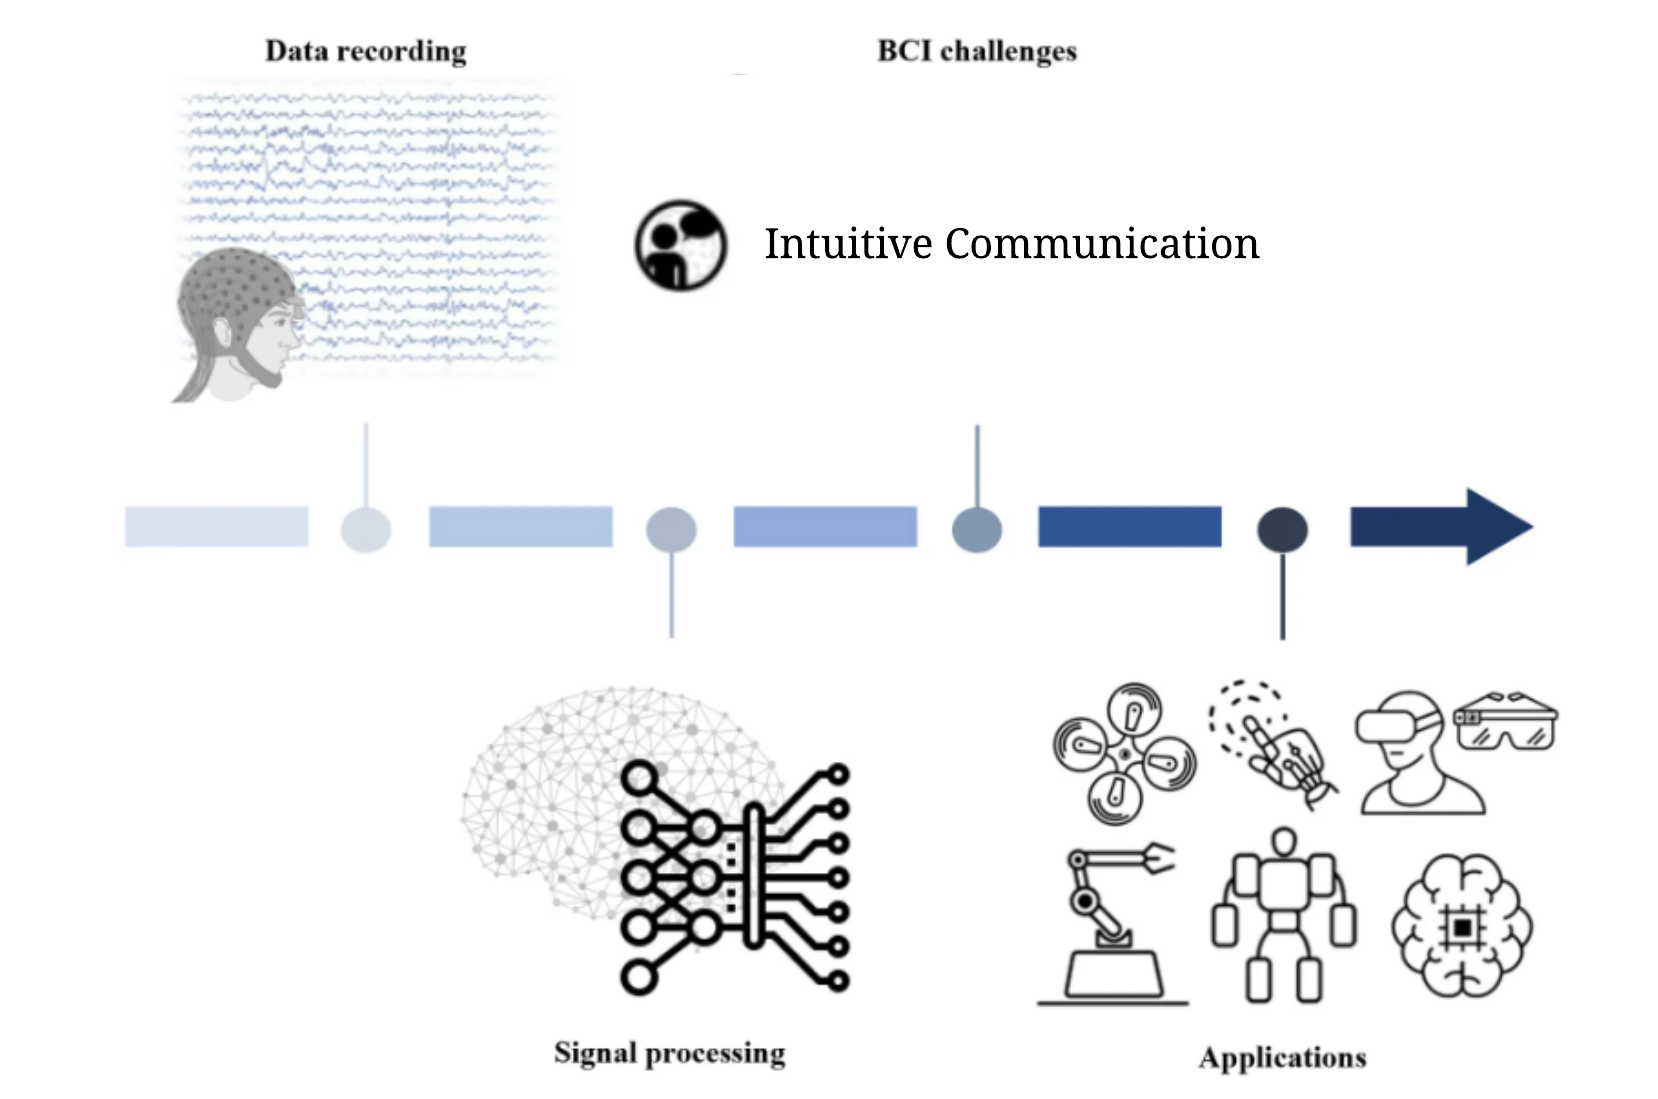
\includegraphics[width=0.8\textwidth]{images/gambar_II_1_bci_flow.png}
  \caption{Alur kerja BCI, mulai dari perekaman data, pemrosesan sinyal, hingga aplikasi, beserta tantangan yang menjadi fokus penelitian ini \parencite[diadaptasi dari][lisensi CC BY]{jeong2022}}
  \label{fig:bci-flow}
\end{figure}

\subsubsection{Perekaman Sinyal Otak}
Sinyal otak dapat direkam dengan beberapa metode yang dikelompokkan berdasarkan aktivitas yang diukur, yaitu listrik (EEG dan ECoG), magnetik (MEG), dan metabolik (fMRI dan fNIRS) \parencite{nicolasalonso2012}.
Perbandingan utamanya ada pada resolusi waktu (seberapa cepat perubahan aktivitas dapat terbaca), resolusi ruang (seberapa tepat lokasi aktivitas dapat ditentukan), risiko bagi pengguna, dan portabilitas.
Perbandingan ini ditunjukkan pada Tabel~\ref{tab:metode-perekaman}.

\begin{table}[H]
  \centering
  \begin{threeparttable}[t]
    \caption{Perbandingan metode perekaman sinyal otak untuk BCI}
    \label{tab:metode-perekaman}
    \begin{tabularx}{\textwidth}{| l | Y | Y | Y | Y | Y |}
      \hline
      \textbf{Metode} & \textbf{Aktivitas yang diukur} & \textbf{Resolusi waktu (detik)} & \textbf{Resolusi ruang (mm)} & \textbf{Risiko} & \textbf{Portabilitas} \\
      \hline
      EEG   & Listrik  & $\sim$0,05  & $\sim$10 & Non-invasif & Portabel \\
      MEG   & Magnetik & $\sim$0,05  & $\sim$5  & Non-invasif & Tidak portabel \\
      ECoG  & Listrik  & $\sim$0,003 & $\sim$1  & Invasif     & Portabel \\
      fMRI  & Metabolik & $\sim$1    & $\sim$1  & Non-invasif & Tidak portabel \\
      fNIRS & Metabolik & $\sim$1    & $\sim$5  & Non-invasif & Portabel \\
      \hline
    \end{tabularx}
    \begin{tablenotes}
      \footnotesize
      \item[] Sumber: diolah dari \textcite{nicolasalonso2012}. Nilai resolusi merupakan perkiraan.
    \end{tablenotes}
  \end{threeparttable}
\end{table}

ECoG menghasilkan sinyal paling tajam dari sisi waktu maupun lokasi, tetapi bersifat invasif karena elektrodanya diletakkan di permukaan otak melalui operasi \parencite{nicolasalonso2012}.
fMRI dan fNIRS merekam aktivitas otak lewat perubahan aliran darah sehingga keduanya sama-sama lambat \parencite{frey2014}.
fMRI sangat teliti dari sisi lokasi, tetapi alatnya berukuran besar, mengelilingi seluruh tubuh pengguna, dan berharga sekitar satu juta dolar AS \parencite{frey2014}.
MEG menangkap perubahan sama cepatnya dengan EEG, tetapi alatnya tidak dapat dipindahkan \parencite{nicolasalonso2012}.

Setiap metode punya kompromi, sehingga pemilihannya bergantung pada kebutuhan.
Alat bantu bagi penderita gangguan komunikasi perlu dipakai di samping pasien, tanpa operasi, dan dengan biaya yang terjangkau.
EEG memenuhi syarat tersebut karena merekam sinyal dari kulit kepala, dapat dibawa, dan menangkap perubahan sinyal dengan cepat \parencite{nicolasalonso2012}.
Dibandingkan alat perekam otak lainnya, EEG dinilai memberikan kompromi terbaik antara ketelitian, kepraktisan, dan biaya \parencite{frey2014}.

Kelemahan EEG adalah ketelitian lokasinya yang lebih rendah, yaitu sekitar 10 mm \parencite{nicolasalonso2012}.
Sinyalnya juga lemah dan mudah tercampur gangguan dari otot dan gerakan mata, sehingga membaca sinyal otak saat \textit{imagined speech} (Subbab~\ref{sec:imagined-speech}) dari EEG masih sulit \parencite{lopezbernal2022}.
Kelemahan ini diterima karena kebutuhan utamanya adalah kepraktisan bagi pasien, dan akan diatasi melalui pengolahan sinyal dan model yang dijelaskan pada subbab berikutnya.

\subsubsection{Pemrosesan Sinyal}
\label{sec:pemrosesan-sinyal}
Sinyal EEG mentah mengandung banyak gangguan sehingga perlu dibersihkan sebelum dipakai.
Gangguan yang umum adalah artefak, yaitu sinyal yang tidak berasal dari aktivitas otak yang dimaksud, misalnya dari kedipan mata dan gerakan otot \parencite{urigue2015}.
Pra-pemrosesan juga menjadi salah satu fokus utama dalam tinjauan penelitian \textit{imagined speech} berbasis EEG \parencite{lopezbernal2022}.

Selain bersih, data juga harus seragam.
Model pembelajaran mesin umumnya menerima masukan dengan ukuran tetap, sehingga seluruh rekaman perlu memiliki jumlah \textit{channel}, \textit{sampling rate}, panjang rekaman, dan rentang amplitudo yang sama.
Rekaman dari subjek, sesi, atau \textit{dataset} yang berbeda sering kali berbeda dalam hal-hal tersebut, misalnya karena alat perekam yang tidak sama.
Istilah \textit{channel} dan \textit{sampling rate} dijelaskan pada Subbab~\ref{sec:cara-kerja-eeg}.

\textcite{zhou2025} memakai rangkaian langkah yang umum untuk mencapai keseragaman itu.
Pertama, \textit{band-pass filter} menahan frekuensi yang terlalu rendah (pergeseran lambat) dan terlalu tinggi (gangguan acak).
Kedua, \textit{notch filter} membuang dengung listrik dari jaringan listrik.
Ketiga, sinyal diubah ke \textit{sampling rate} yang sama (\textit{resampling}).
Keempat, amplitudo sinyal diskalakan ke rentang yang sama agar nilainya seragam antar rekaman.

Penyamaan \textit{sampling rate} ke nilai yang lebih rendah perlu didahului \textit{low-pass filter}, yaitu penyaring yang membuang frekuensi tinggi, agar tidak muncul gangguan \textit{aliasing}, yaitu frekuensi tinggi yang terbaca sebagai frekuensi rendah yang palsu \parencite{oppenheim2010}.
Jumlah \textit{channel} dapat disamakan dengan memilih \textit{channel} yang dimiliki semua rekaman.
Setelah itu, sinyal dipotong menjadi percobaan (\textit{trial}), yaitu potongan sinyal untuk satu kata, sesuai rentang waktu saat subjek membayangkannya.
Penyeragaman sinyal antar subjek dibahas pada Subbab~\ref{sec:rct}, dan pemetaan sinyal ke vektor makna dibahas pada Subbab~\ref{sec:vektor-makna}.

\subsubsection{Tantangan BCI}
BCI masih memiliki banyak tantangan yang berbeda-beda.
Kompetisi BCI internasional 2020 mengangkat lima tantangan teknis, masing-masing dengan \textit{dataset}-nya sendiri \parencite{jeong2022}.
Pertama, \textit{few-shot EEG learning}, yaitu belajar dari data kalibrasi yang sangat sedikit untuk setiap pengguna.
Kedua, \textit{micro-sleep detection}, yaitu mendeteksi tidur yang sangat singkat dari satu \textit{channel}.
Ketiga, \textit{imagined speech decoding} untuk komunikasi BCI yang intuitif (\textit{intuitive communication}), yaitu pengguna menyampaikan kata atau frasa utuh secara langsung, bukan mengeja huruf satu per satu.
Keempat, \textit{cross-session classification} gerakan lengan atas, yaitu menjaga ketepatan model walaupun sinyal direkam pada sesi yang berbeda.
Kelima, deteksi ERP pada kondisi bergerak (\textit{ambulatory environment}), yaitu perekaman saat pengguna tidak duduk diam di laboratorium.

Dari lima tantangan tersebut, penelitian ini hanya akan berfokus pada komunikasi yang membaca maksud pengguna dari pikirannya tanpa stimulus dari luar.
Bentuk yang dipilih adalah \textit{imagined speech}, yaitu pengguna membayangkan mengucapkan kata dalam hati.

\subsubsection{Aplikasi BCI}
Hasil terjemahan sinyal otak diteruskan ke aplikasi, yaitu perangkat yang menjalankan perintah atau menyampaikan informasi dari pengguna \parencite{nicolasalonso2012}.
Aplikasi BCI beragam, misalnya mengendalikan robot, \textit{drone}, dan perangkat realitas virtual seperti pada Gambar~\ref{fig:bci-flow}.

Dalam penelitian ini, aplikasi yang dituju adalah alat bantu komunikasi bagi orang yang tidak dapat berbicara.
Penderita gangguan saraf dan otot berat seperti ALS dan stroke batang otak bisa saja tahu apa yang ingin disampaikan, tetapi kesulitan mengeluarkannya lewat ucapan maupun tulisan \parencite{wolpaw2002}.
Setelah stroke, hingga 40\% penderita mengalami afasia, yaitu gangguan berbahasa akibat kerusakan jaringan bahasa di otak \parencite{cochrane2025}.

\subsection{\textit{Imagined Speech}}
\label{sec:imagined-speech}
\textit{Imagined speech} adalah kondisi ketika seseorang membayangkan mengucapkan sebuah kata dalam hati tanpa menggerakkan mulut atau bersuara, dan sinyal EEG pada saat itu direkam untuk dibaca.
Sinyal ini dapat menjadi jalur komunikasi baru bagi orang yang tidak mampu berbicara akibat disabilitas motorik atau penyakit saraf \parencite{lopezbernal2022}.
Pendekatan yang umum digunakan adalah klasifikasi, yaitu model dilatih untuk memilih satu kata dari daftar kata target yang sudah ditentukan sebelumnya \parencite{lopezbernal2022}.
Selain klasifikasi ke daftar kata tetap, ada pendekatan lain yang memetakan sinyal otak ke representasi makna \parencite{tang2023}, yang dibahas pada Subbab~\ref{sec:vektor-makna}.

Hasil klasifikasi \textit{imagined speech} sangat bergantung pada jenis tugasnya.
Menurut \textcite{duhair2026}, tugas dengan dua pilihan sering melaporkan akurasi di atas 80 persen, tetapi pengenalan kata atau fonem dengan banyak pilihan memberikan hasil yang sangat beragam dan peka terhadap rancangan \textit{dataset} serta cara pengujian.

Ada tiga tantangan utama.
Pertama, sinyal EEG saat \textit{imagined speech} memiliki rasio sinyal terhadap gangguan (\textit{signal-to-noise ratio} atau SNR) yang rendah \parencite{lopezbernal2022}.
Kedua, sinyal berbeda cukup besar antar orang, sementara data yang tersedia masih kecil dan beragam \parencite{duhair2026}.
Ketiga, metode invasif seperti ECoG rata-rata menghasilkan akurasi klasifikasi yang lebih tinggi daripada metode non-invasif \parencite{lopezbernal2022}.

% ============================================================================================
% II.2 EEG
% ============================================================================================
\section{EEG}
\subsection{Cara Kerja EEG}
\label{sec:cara-kerja-eeg}
EEG merekam aktivitas listrik otak lewat elektroda yang ditempelkan di kulit kepala.
Penempatan elektroda umumnya mengikuti sistem internasional 10-20, yaitu jarak antar elektroda diatur pada kelipatan 10 atau 20 persen dari jarak depan-belakang dan kiri-kanan kepala \parencite{britton2016}.
Nama setiap elektroda terdiri atas huruf dan angka.
Huruf menunjukkan bagian otak di bawahnya (F untuk frontal, T untuk temporal, P untuk parietal, dan O untuk oksipital), angka ganjil berada di sisi kiri kepala, angka genap di sisi kanan, dan huruf z di garis tengah \parencite{britton2016}.
Setiap elektroda menghasilkan satu rangkaian sinyal yang disebut \textit{channel}, seperti terlihat pada Gambar~\ref{fig:posisi-elektroda}.

\begin{figure}[H]
  \centering
  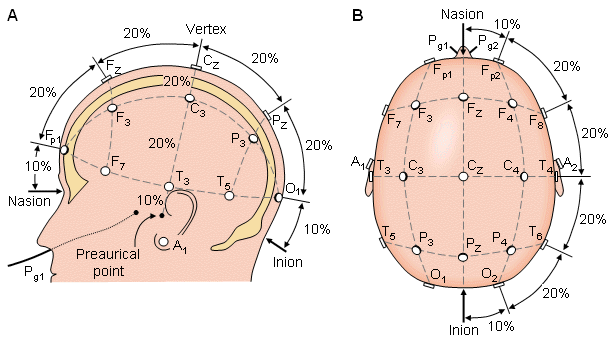
\includegraphics[width=0.8\textwidth]{images/gambar_II_2_posisi_elektroda.png}
  \caption{Sistem internasional 10-20 dilihat dari kiri (A) dan atas kepala (B) \parencite[sumber:][]{malmivuo1995}}
  \label{fig:posisi-elektroda}
\end{figure}

Sinyal EEG dikelompokkan menurut frekuensinya, yaitu jumlah gelombang per detik dengan satuan Hz.
Gelombang delta berfrekuensi 1 sampai 3 Hz, theta 4 sampai 7 Hz, alpha 8 sampai 12 Hz, dan beta 13 Hz ke atas, sedangkan frekuensi di atas 25 Hz (gamma) jarang terlihat pada EEG kulit kepala \parencite{britton2016}.
Rekaman EEG berupa deretan angka untuk setiap \textit{channel} pada setiap titik waktu, dan jumlah titik data yang diambil per detik disebut \textit{sampling rate}.

\subsection{\textit{Dataset} EEG \textit{Imagined Speech}}
\label{sec:dataset-eeg}
Salah satu \textit{dataset} publik untuk \textit{imagined speech} adalah BCI Competition 2020-3, yang dirilis dalam kompetisi BCI internasional 2020 \parencite{jeong2022}.
Sebanyak 15 subjek diminta membayangkan lima kata atau frasa, yaitu \textit{“hello”}, \textit{“help me”}, \textit{“stop”}, \textit{“thank you”}, dan \textit{“yes”}.
EEG direkam dari 64 \textit{channel} dengan \textit{sampling rate} 256 Hz, dan setiap sampel berupa rekaman selama 3 detik \parencite{zhou2025}.

Pembagian data ditentukan oleh kompetisi.
Untuk setiap subjek tersedia 60 percobaan per kata untuk pelatihan, 10 untuk validasi, dan 10 untuk pengujian, sehingga totalnya 6.000 percobaan \parencite{jeong2022,zhou2025}.


% ============================================================================================
% II.3 RCT
% ============================================================================================
\section{Penyeragaman Sinyal Antar Subjek dengan RCT}
\label{sec:rct}
Sinyal EEG untuk kata yang sama berbeda cukup besar dari satu orang ke orang lain \parencite{duhair2026}, sehingga model yang dilatih pada satu orang sulit dipakai pada orang lain.
Salah satu cara mengatasinya adalah \textit{transfer learning} berbasis geometri Riemann.
Cara ini merepresentasikan data lewat matriks kovarians spasial, lalu menggeser data setiap subjek ke acuan yang sama agar data antar subjek dapat dibandingkan \parencite{zanini2018}.
Dalam proposal ini, pemusatan tersebut disebut \textit{Riemannian Centering Transformation} (RCT).

Matriks kovarians spasial adalah tabel berukuran $N \times N$, dengan $N$ jumlah \textit{channel}, yang menunjukkan seberapa kuat setiap pasang \textit{channel} naik dan turun bersamaan.
Untuk satu percobaan dengan sinyal $X$ berukuran $N$ \textit{channel} $\times$ $T$ titik waktu, matriks ini dihitung dengan Persamaan~\ref{eq:kovarians}.
Karena waktu sudah diringkas, ukuran matriksnya tetap $N \times N$ berapa pun panjang rekaman.
\begin{equation}
C_i = \frac{1}{T-1}\, X_i X_i^{\top}
\label{eq:kovarians}
\end{equation}
\eqcaption{Matriks kovarians spasial}

Matriks kovarians tidak berada pada ruang datar biasa, melainkan pada ruang lengkung yang disebut \textit{manifold} Riemann.
Karena itu, rata-rata yang tepat adalah rata-rata Riemann (rata-rata geometrik), yaitu matriks yang meminimalkan jumlah kuadrat jarak Riemann ke semua matriks lainnya \parencite{he2020}, seperti pada Persamaan~\ref{eq:rata-riemann}.
Pemusatan kemudian dilakukan dengan Persamaan~\ref{eq:pemusatan}, sehingga rata-rata baru setiap subjek menjadi matriks identitas \parencite{zanini2018}.
\begin{equation}
\bar{C} = \arg\min_{C \succ 0} \sum_{i=1}^{M} \delta_R^{2}(C, C_i)
\label{eq:rata-riemann}
\end{equation}
\eqcaption{Rata-rata Riemann}

\begin{equation}
\tilde{C}_i = \bar{C}^{-1/2}\, C_i\, \bar{C}^{-1/2}
\label{eq:pemusatan}
\end{equation}
\eqcaption{Pemusatan matriks kovarians}

Pada persamaan tersebut, $M$ adalah jumlah percobaan satu subjek, $\delta_R$ adalah jarak Riemann, dan $\bar{C}$ adalah rata-rata Riemann milik subjek itu.
Operasi ini setara dengan \textit{whitening}, yaitu penyeragaman sebaran sinyal, memakai rata-rata Riemann \parencite{bleuze2022}.
Jarak antar matriks pada subjek yang sama tidak berubah, tetapi data setiap subjek bergeser ke titik acuan yang sama sehingga lebih mudah dibandingkan \parencite{he2020}.
Prosesnya tidak memerlukan label kata, tetapi memerlukan sejumlah rekaman dari subjek tersebut untuk menghitung rata-ratanya.
Ilustrasi pemusatan ditunjukkan pada Gambar~\ref{fig:rct}.

\begin{figure}[H]
  \centering
  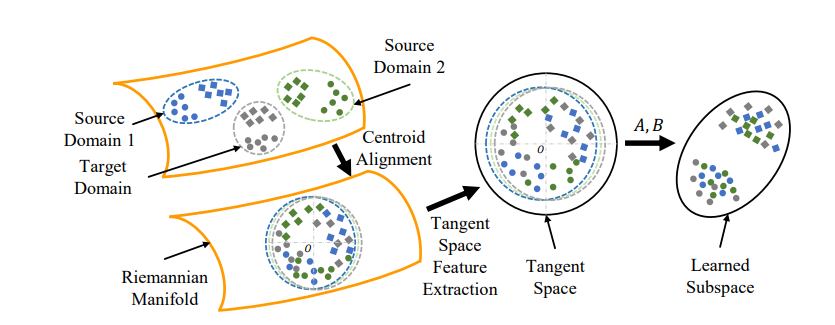
\includegraphics[width=0.9\textwidth]{images/gambar_II_3_rct.png}
  \caption{Alur MEKT: penyelarasan pusat data pada \textit{manifold} Riemann, pemetaan ke \textit{tangent space}, lalu pembelajaran subruang \parencite[sumber:][]{zhang2020}}
  \label{fig:rct}
\end{figure}

Banyak model pembelajaran mesin menerima masukan berupa vektor, sehingga matriks kovarians yang sudah dipusatkan perlu diubah menjadi vektor terlebih dahulu.
Salah satu caranya adalah memetakan matriks tersebut ke \textit{tangent space}, yaitu ruang datar di sekitar titik acuan \parencite{barachant2012}.
\textcite{zanini2018} menguji pemusatan ini pada BCI gerakan yang dibayangkan (\textit{motor imagery}) dan respons potensial otak (ERP), sedangkan penerapannya pada \textit{imagined speech} belum ditemukan pada literatur yang ditelaah dalam studi ini.

% ============================================================================================
% II.4 Vektor makna
% ============================================================================================
\section{Vektor Makna dan Pemetaan EEG ke Vektor}
\label{sec:vektor-makna}
\subsection{Vektor Makna}
Komputer tidak membaca makna dari huruf.
Cara umum untuk menyampaikan makna ke komputer adalah mengubah data, misalnya kata atau kalimat, menjadi vektor, yaitu deretan angka, yang disebut \textit{embedding}.
Kata atau kalimat yang maknanya dekat mendapat vektor yang berdekatan \parencite{reimers2019}.
\textcite{pereira2018} menyebut ruang tempat vektor-vektor ini berada sebagai ruang semantik, yang dibangun dari kumpulan teks yang sangat besar.

Konsep \textit{embedding} tidak terbatas pada teks.
Gambar, misalnya, dapat diubah menjadi vektor oleh model CLIP \parencite{mokady2021}, dan data pencitraan otak dapat dipetakan ke vektor dalam ruang semantik yang sama dengan teks \parencite{pereira2018}.
Dengan cara ini, sinyal otak dan kata dapat dibandingkan dalam satu ruang vektor, sehingga kedekatan maknanya dapat diukur dengan ukuran yang sama.

Kedekatan dua vektor, baik yang berasal dari teks maupun dari sinyal, diukur dengan \textit{cosine similarity}, seperti pada Persamaan~\ref{eq:cosine} dan diilustrasikan pada Gambar~\ref{fig:ruang-makna}.
Nilainya 1 bila arah kedua vektor sama persis, yang berarti maknanya sangat dekat, dan makin kecil bila maknanya makin berbeda.
Ukuran ini memberi nilai kedekatan yang bertingkat, bukan sekadar benar atau salah.
\begin{equation}
\cos(\mathbf{a}, \mathbf{b}) = \frac{\mathbf{a} \cdot \mathbf{b}}{\lVert \mathbf{a} \rVert \, \lVert \mathbf{b} \rVert}
\label{eq:cosine}
\end{equation}
\eqcaption{\textit{Cosine similarity}}

\begin{figure}[H]
  \centering
  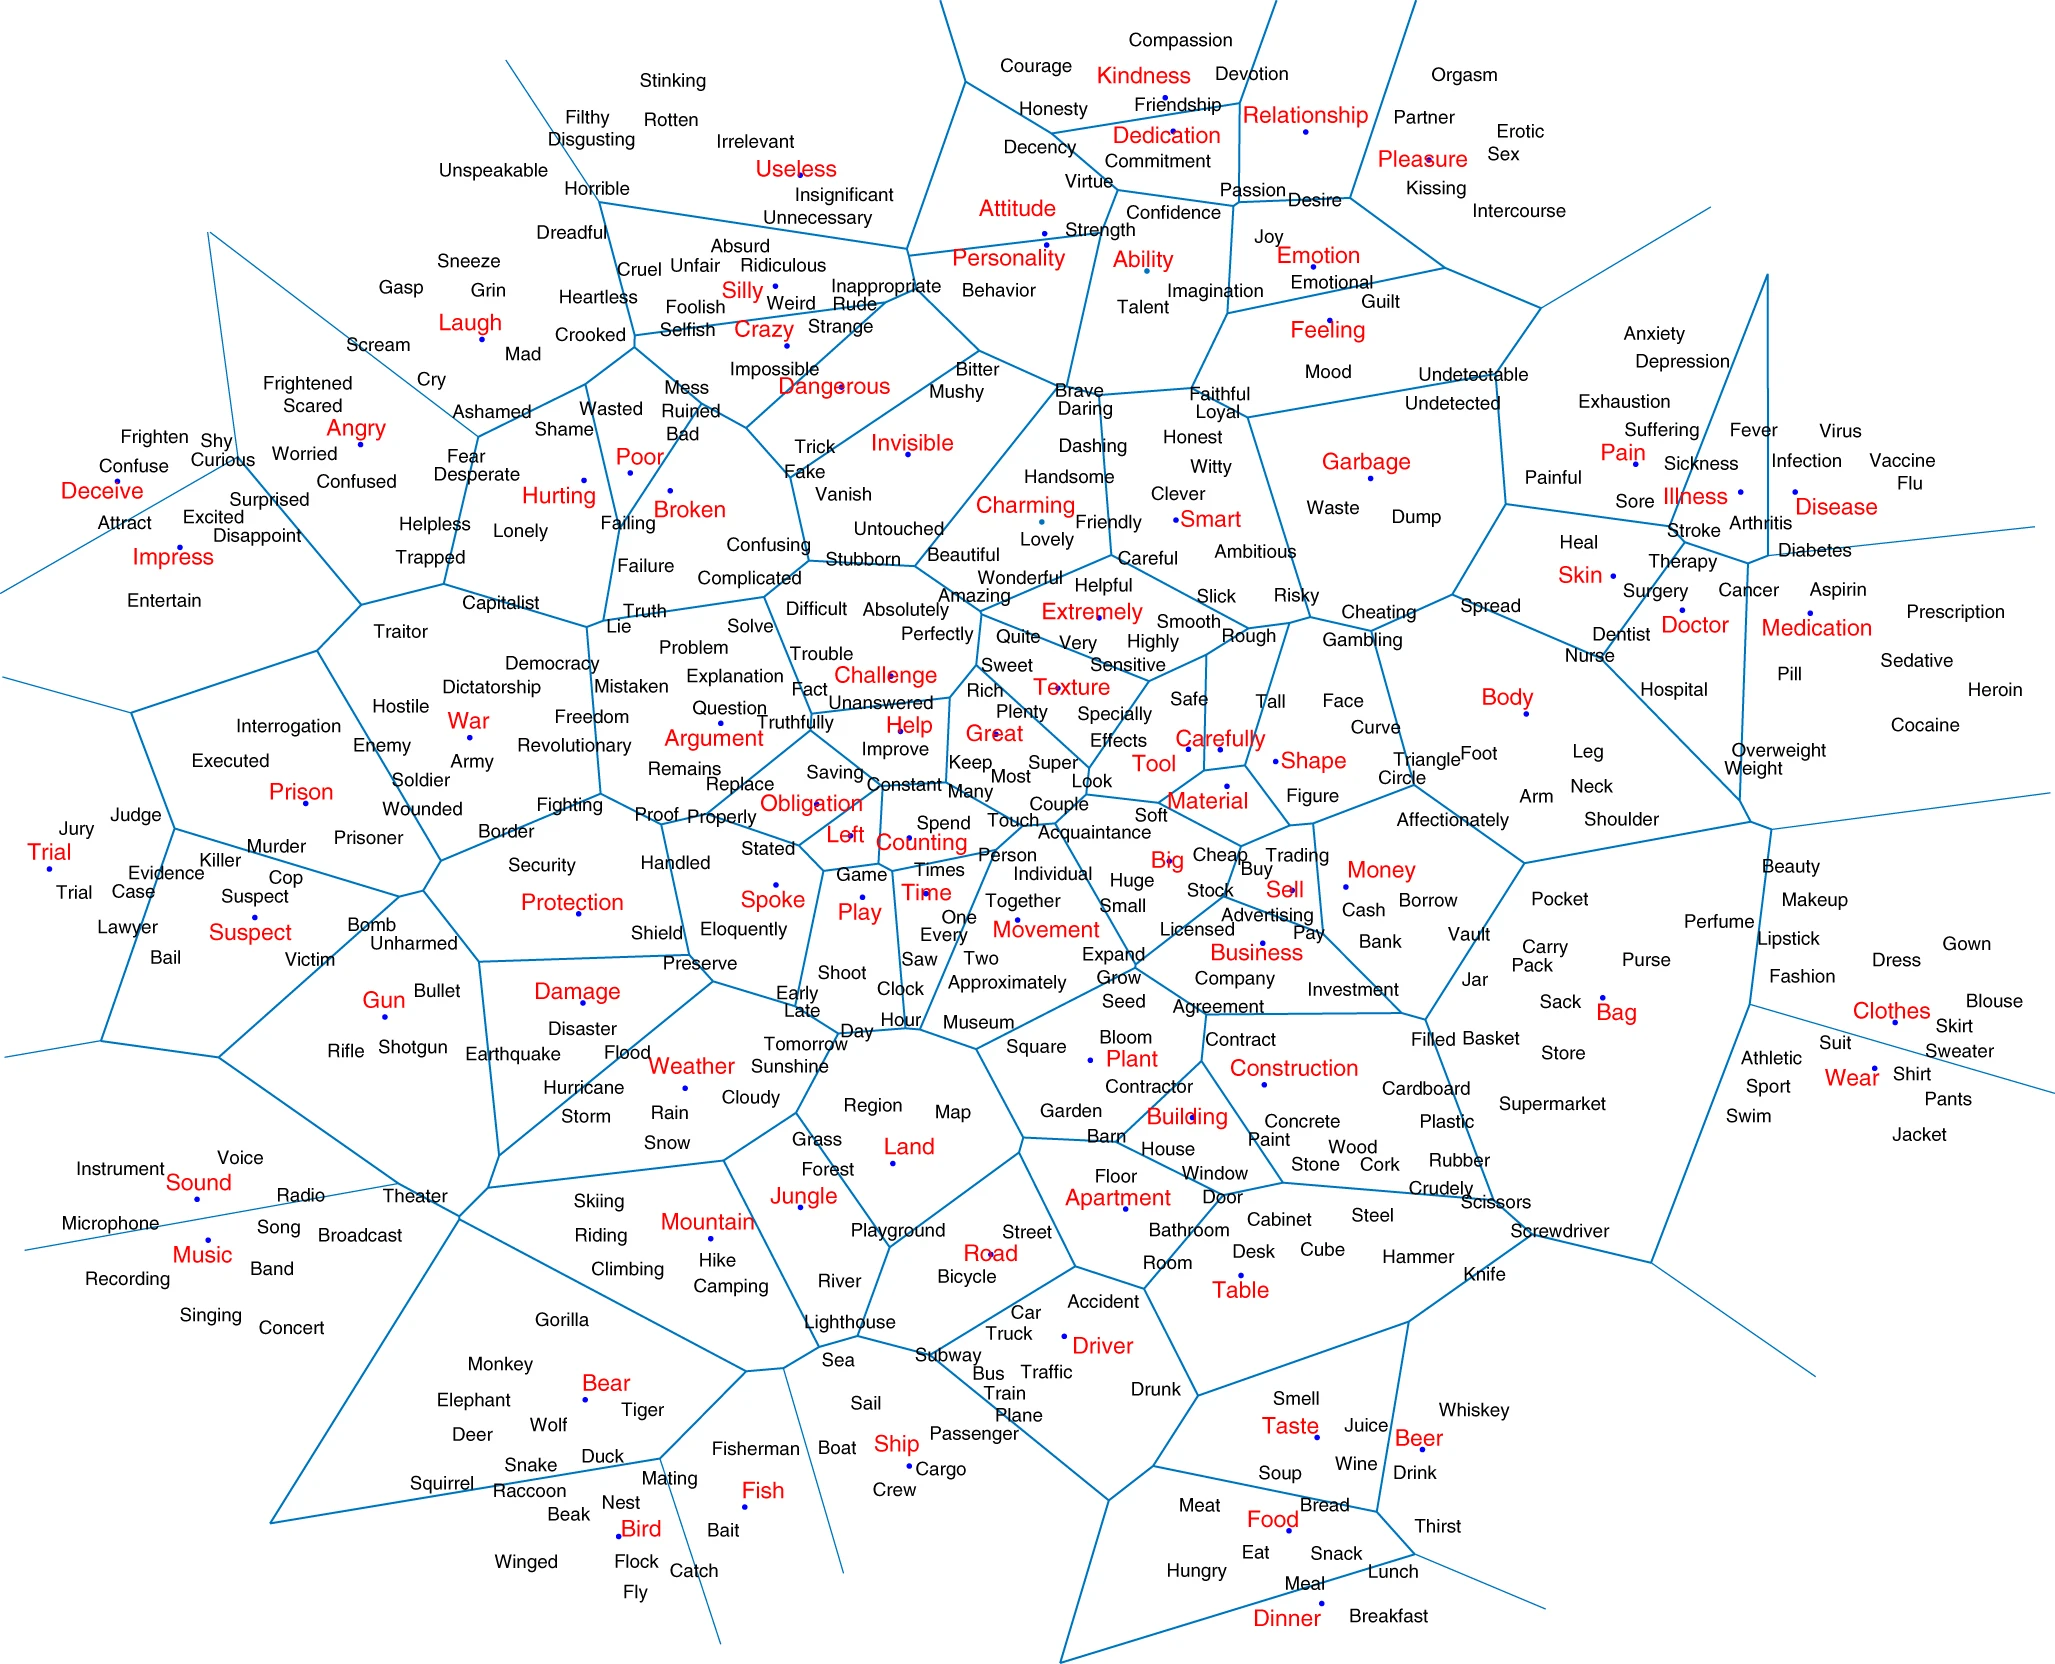
\includegraphics[width=0.85\textwidth]{images/gambar_II_4_ruang_vektor_makna.png}
  \caption{Ilustrasi ruang semantik dua dimensi, dengan kata-kata yang maknanya berdekatan membentuk kelompok \parencite[sumber:][]{pereira2018}}
  \label{fig:ruang-makna}
\end{figure}

\subsection{Model \textit{Sentence Embedding}}
Vektor makna dihasilkan oleh model \textit{embedding}.
Model \textit{sentence embedding} menghasilkan satu vektor berukuran tetap untuk satu kalimat atau frasa dengan panjang berapa pun, sehingga teks yang berbeda panjang dapat dibandingkan dalam ruang vektor yang sama \parencite{reimers2019}.

Salah satu pendekatan \textit{sentence embedding} adalah Sentence-BERT (SBERT), yaitu modifikasi dari jaringan BERT yang sudah dilatih sebelumnya.
BERT sendiri tidak menghasilkan vektor kalimat yang berdiri sendiri, sehingga sulit dipakai untuk mencari kalimat yang maknanya mirip \parencite{reimers2019}.
SBERT menambahkan operasi \textit{pooling}, misalnya merata-ratakan vektor semua \textit{token} keluaran BERT, untuk mendapat satu vektor berukuran tetap.
Jaringan itu kemudian dilatih ulang dengan struktur \textit{siamese} dan \textit{triplet}, yaitu dua atau tiga salinan jaringan dengan bobot yang sama yang dipasangkan pada pasangan kalimat, agar kalimat yang maknanya mirip berdekatan dalam ruang vektor dan dapat dibandingkan dengan \textit{cosine similarity} \parencite{reimers2019}.
Arsitektur SBERT saat menghitung kemiripan dua kalimat ditunjukkan pada Gambar~\ref{fig:sbert}.

\begin{figure}[H]
  \centering
  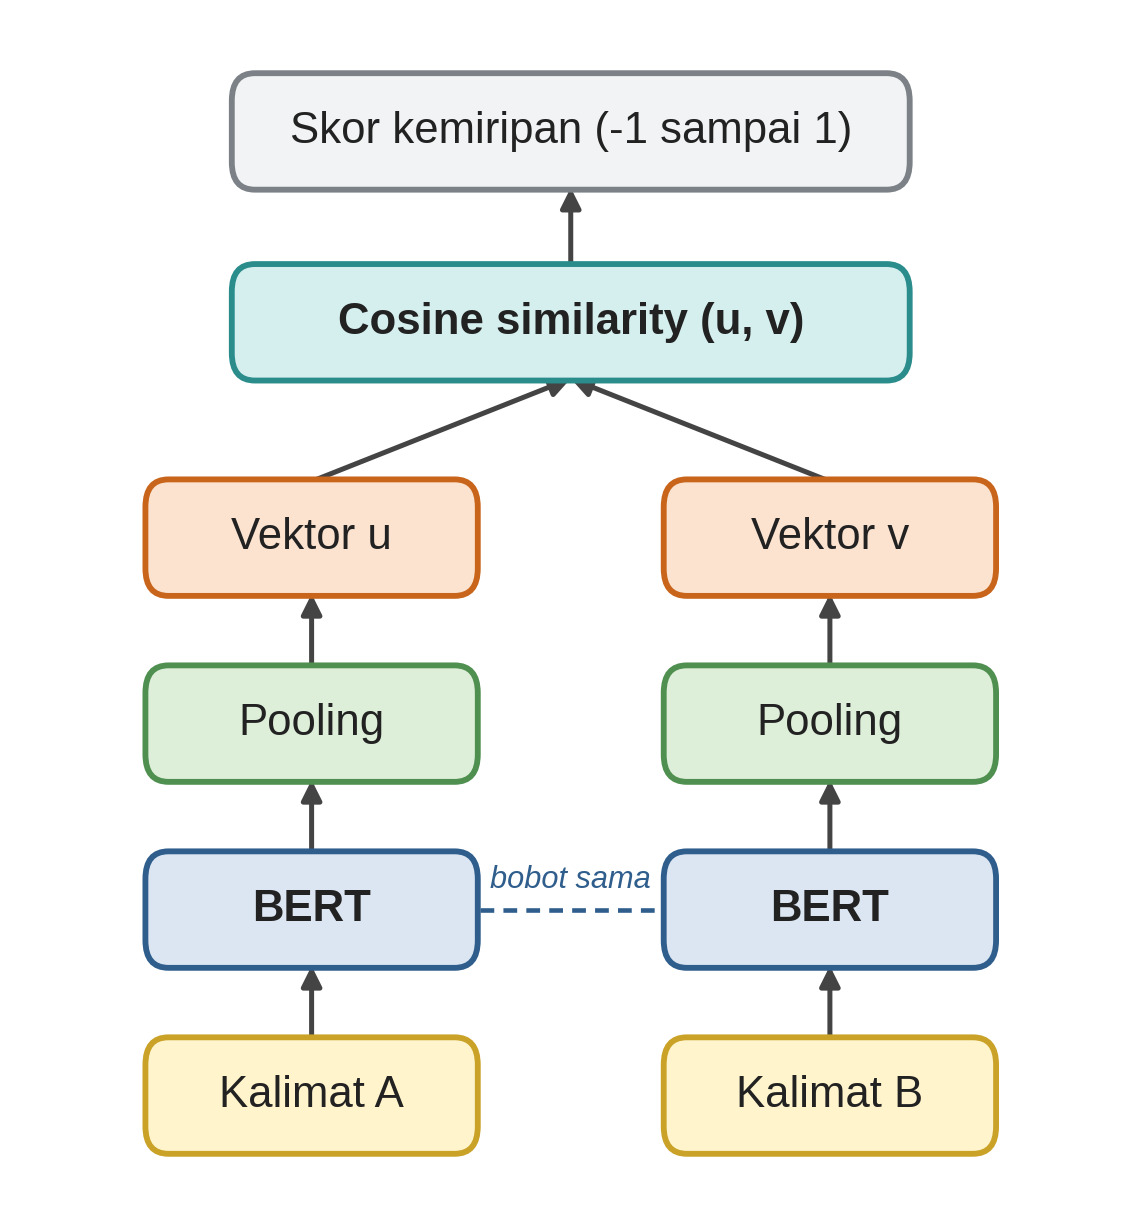
\includegraphics[width=0.6\textwidth]{images/gambar_II_5_sbert_kemiripan.png}
  \caption{Arsitektur SBERT saat menghitung kemiripan dua kalimat \parencite[diadaptasi dari][]{reimers2019}}
  \label{fig:sbert}
\end{figure}

\subsection{Pemetaan Sinyal Otak ke Vektor Makna}
\textcite{pereira2018} membangun \textit{decoder} yang memetakan data pencitraan otak ke vektor dalam ruang semantik.
\textit{Decoder} dilatih dari data konsep tunggal, lalu mampu mengenali makna kalimat baru dengan topik yang tidak muncul saat pelatihan, dan hasilnya menangkap struktur kemiripan makna antar kalimat.
\textcite{tang2023} melanjutkan arah ini dengan merekonstruksi bahasa secara berkelanjutan, sehingga menghasilkan rangkaian kata yang maknanya sesuai dengan ucapan yang dibayangkan seseorang.
Kedua penelitian tersebut memakai data pencitraan otak fMRI, bukan EEG.

Pemetaan dari sinyal otak ke vektor makna pada dasarnya adalah masalah regresi, yaitu memprediksi angka-angka penyusun vektor makna dari fitur sinyal.
Model belajar dari pasangan data berupa fitur sinyal dan vektor makna dari kata yang sedang diproses otak, dengan meminimalkan selisih antara vektor prediksi dan vektor target, seperti pada Persamaan~\ref{eq:regresi}.
Bentuk modelnya beragam, mulai dari regresi linear sampai jaringan saraf.
\begin{equation}
\hat{\theta} = \arg\min_{\theta} \sum_{i=1}^{M} \lVert \mathbf{y}_i - f_{\theta}(\mathbf{x}_i) \rVert_2^{2}
\label{eq:regresi}
\end{equation}
\eqcaption{Pelatihan model pemetaan sinyal ke vektor makna}

Pada persamaan tersebut, $M$ adalah jumlah percobaan, $\mathbf{x}_i$ adalah fitur sinyal pada percobaan ke-$i$, $\mathbf{y}_i$ adalah vektor makna targetnya, $f_{\theta}$ adalah model dengan parameter $\theta$, dan $\hat{\theta}$ adalah parameter terbaik hasil pelatihan.
Vektor hasil prediksi dapat diterjemahkan kembali menjadi kata dengan mencari kata kandidat yang vektornya paling dekat menurut \textit{cosine similarity}.

% ============================================================================================
% II.5 SAE
% ============================================================================================
\section{\textit{Sparse Autoencoder} (SAE)}
\textit{Autoencoder} adalah jaringan saraf yang belajar mengubah sebuah vektor menjadi bentuk lain, lalu mengembalikannya sedekat mungkin ke vektor semula.
Pada \textit{sparse autoencoder} (SAE), bentuk di tengahnya dibuat lebih lebar daripada vektor asli, tetapi hanya sedikit angka yang boleh aktif pada satu waktu \parencite{bricken2023,cunningham2023}.
Pelatihannya meminimalkan galat rekonstruksi ditambah penalti pada jumlah angka yang aktif, seperti pada Persamaan~\ref{eq:sae}.
\begin{equation}
\mathcal{L} = \lVert \mathbf{x} - \hat{\mathbf{x}} \rVert_2^{2} + \alpha \lVert \mathbf{f} \rVert_1
\label{eq:sae}
\end{equation}
\eqcaption{Fungsi galat \textit{sparse autoencoder}}

Pada persamaan tersebut, $\mathbf{x}$ adalah vektor masukan, $\mathbf{f}$ adalah angka-angka di lapisan tengah yang lebih lebar, $\hat{\mathbf{x}}$ adalah hasil rekonstruksi, dan $\alpha$ adalah kekuatan penalti agar sedikit angka yang aktif.

SAE digunakan dalam penelitian interpretabilitas model bahasa karena sebuah dimensi pada vektor sering aktif untuk beberapa makna yang tidak berhubungan, yang disebut polisemantik.
Salah satu dugaan penyebabnya adalah superposisi, yaitu jaringan menyimpan lebih banyak ciri daripada jumlah dimensinya dengan menempatkannya pada arah-arah yang saling tumpang tindih \parencite{cunningham2023}.
SAE memisahkan arah-arah ini, dan hasilnya berupa ciri yang lebih mudah ditafsirkan dan lebih bersifat satu makna dibandingkan metode pembanding \parencite{cunningham2023,bricken2023}.
Penerapan SAE yang dilaporkan pada kedua penelitian tersebut adalah pada aktivasi di dalam model bahasa.
Struktur SAE ditunjukkan pada Gambar~\ref{fig:sae}.

\begin{figure}[H]
  \centering
  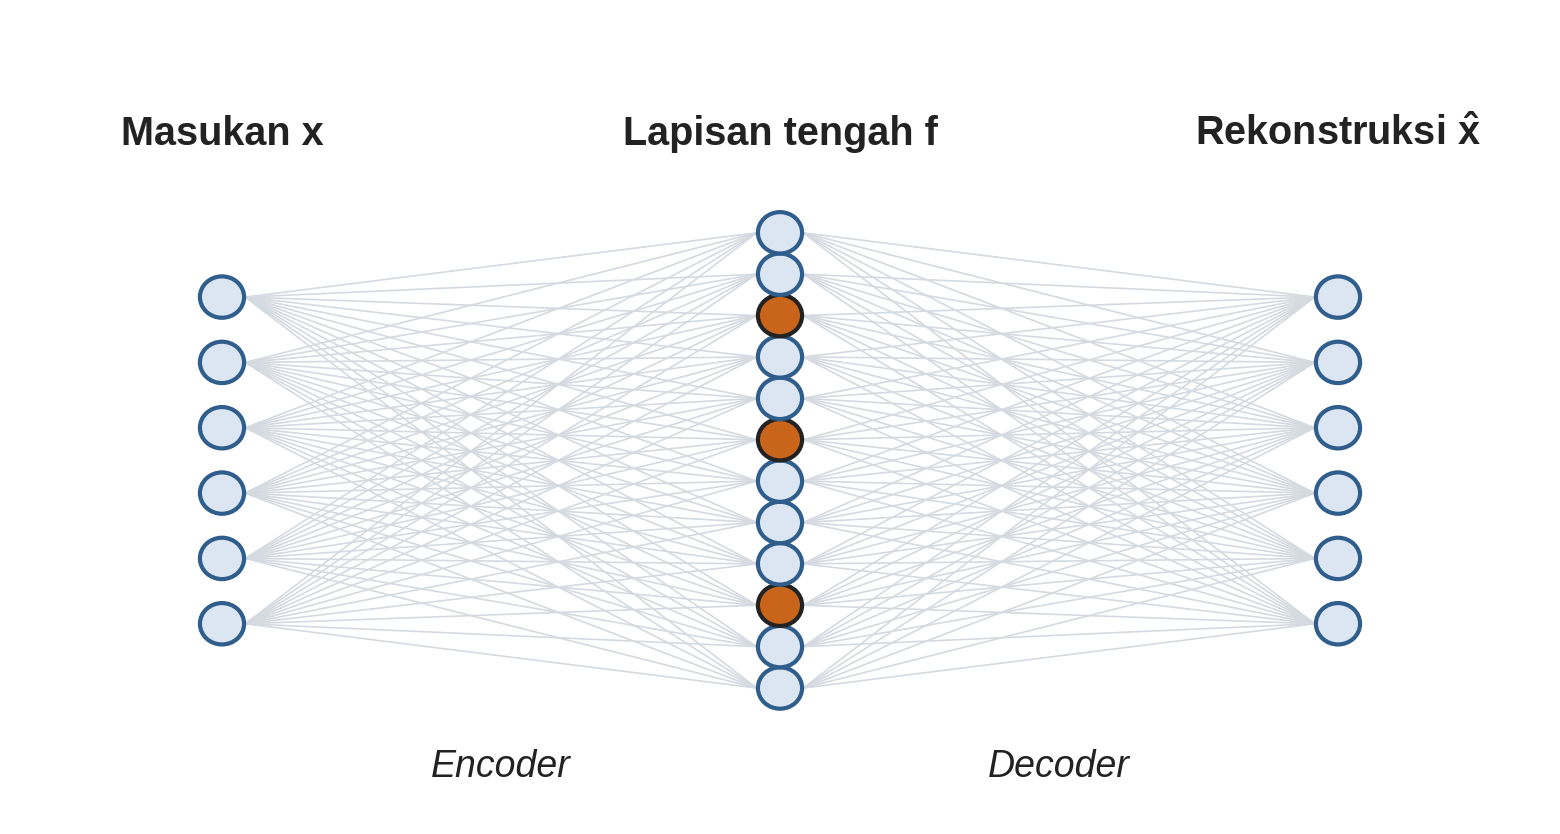
\includegraphics[width=0.8\textwidth]{images/gambar_II_6_sae.png}
  \caption{Ilustrasi struktur \textit{sparse autoencoder}, dengan unit yang aktif ditandai warna oranye}
  \label{fig:sae}
\end{figure}

% ============================================================================================
% II.6 LLM
% ============================================================================================
\section{\textit{Large Language Model} (LLM)}
Model bahasa \textit{pretrained} (\textit{pretrained language model}) dibangun dengan melatih model Transformer pada kumpulan teks berskala besar, sehingga mampu menyelesaikan berbagai tugas pemrosesan bahasa.
Istilah \textit{large language model} (LLM) dipakai untuk model \textit{pretrained} yang berukuran besar, misalnya berisi puluhan atau ratusan miliar parameter, yaitu angka-angka yang membentuk model \parencite{zhao2023}.

LLM tidak membaca huruf secara langsung.
Teks dipecah menjadi \textit{token}, yaitu potongan kata, lalu setiap \textit{token} diubah menjadi vektor sebelum diproses \parencite{mokady2021}.
Karena itu, apa yang sebenarnya diterima LLM adalah deretan vektor, dan hal inilah yang memungkinkan vektor diberikan langsung tanpa melalui kata.

% ============================================================================================
% II.7 Soft prompt
% ============================================================================================
\section{\textit{Soft Prompt}}
\textit{Prompt} biasa adalah teks yang diubah menjadi vektor oleh LLM.
\textit{Soft prompt} adalah deretan vektor yang langsung diberikan kepada LLM di depan masukan, tanpa harus ditulis sebagai kata.
Pada \textcite{lester2021}, isi vektor ini dilatih supaya LLM yang dibekukan menjalankan tugas tertentu, bukan dipilih dari kata yang ada, sehingga vektor tersebut mewakili tugas.
Pendekatan serupa, yaitu \textit{prefix-tuning}, menambahkan vektor khusus tugas ke bagian dalam model \parencite{liliang2021}.

Vektor di depan masukan juga dapat dihasilkan oleh jaringan kecil dari masukan lain, sehingga isinya mewakili masukan itu dan bukan hanya tugas, dan isinya berubah pada setiap data \parencite{mokady2021}.
Dalam proposal ini, istilah \textit{soft prompt} dipakai secara luas untuk kedua bentuk tersebut.

\textcite{lester2021} melaporkan bahwa selisih performa antara \textit{soft prompt} dan \textit{fine-tuning} penuh, yaitu melatih ulang seluruh bobot model, mengecil seiring bertambahnya ukuran model.
\textit{Soft prompt} juga lebih ringan karena hanya vektor kecil yang disimpan untuk tiap tugas, sedangkan \textit{fine-tuning} penuh menghasilkan salinan model utuh.
Cara kerja \textit{soft prompt} ditunjukkan pada Gambar~\ref{fig:soft-prompt}.

\begin{figure}[H]
  \centering
  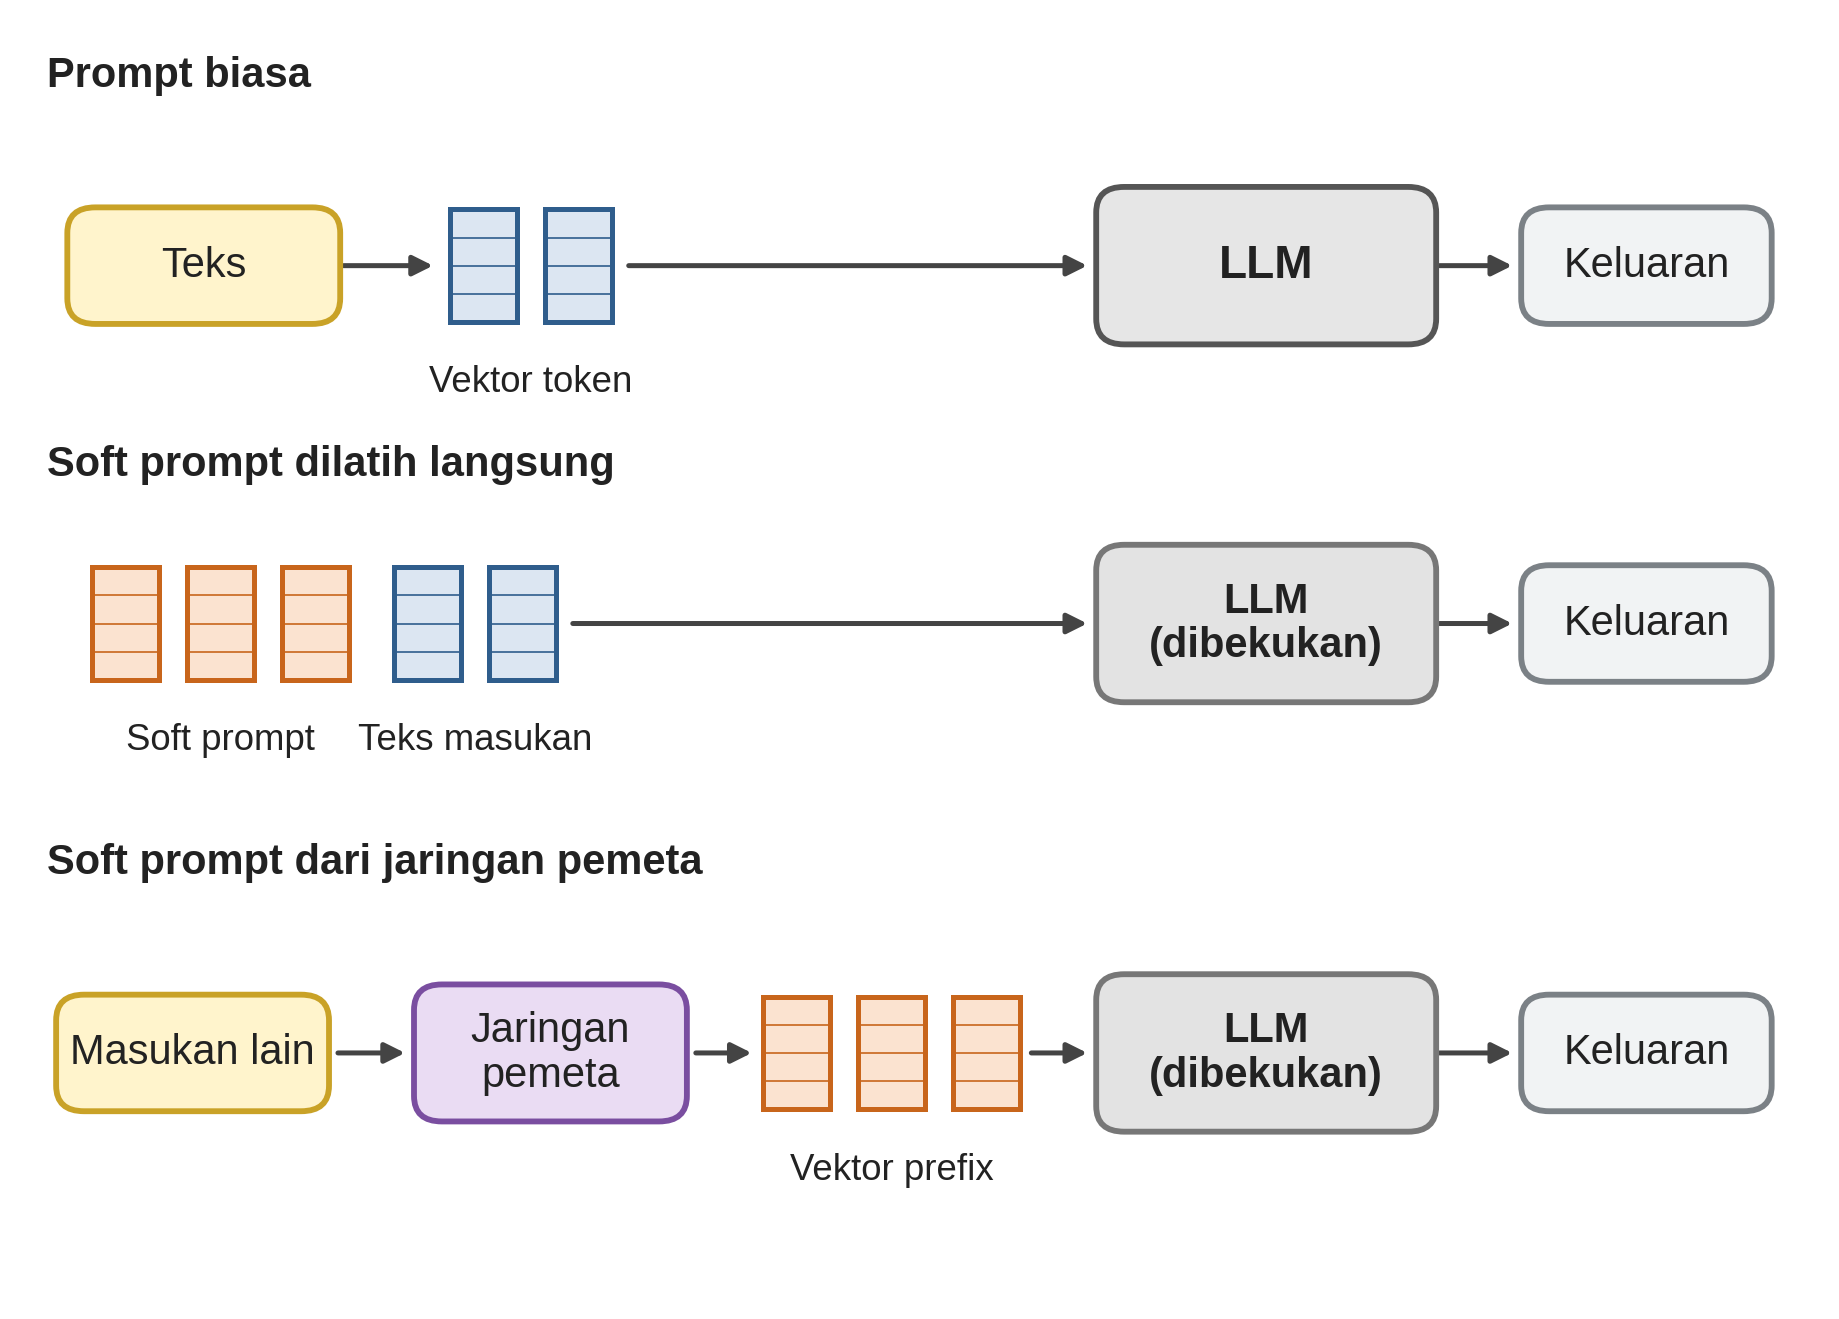
\includegraphics[width=0.9\textwidth]{images/gambar_II_7_soft_prompt.png}
  \caption{Perbandingan \textit{prompt} biasa dan dua bentuk \textit{soft prompt} (diadaptasi dari \citeauthor{lester2021}, \citeyear{lester2021}; \citeauthor{mokady2021}, \citeyear{mokady2021})}
  \label{fig:soft-prompt}
\end{figure}

% ============================================================================================
% II.8 Adapter
% ============================================================================================
\section{\textit{Adapter}}
Vektor dari satu model \textit{embedding} tidak berada di ruang yang sama dengan vektor kata di dalam LLM, dan ukurannya pun berbeda.
\textit{Adapter} adalah jaringan kecil yang menerjemahkan vektor dari satu ruang ke ruang masukan LLM.
Pada ClipCap, jaringan pemeta ringan mengubah \textit{embedding} gambar menjadi sejumlah vektor yang berukuran sama dengan \textit{embedding} kata, lalu menaruhnya di depan teks sebagai \textit{prefix} untuk GPT-2 \parencite{mokady2021}.

\textcite{mokady2021} juga melaporkan bahwa metode ini tetap bekerja walaupun hanya jaringan pemeta yang dilatih, sementara model pembuat \textit{embedding} gambar dan model bahasanya dibekukan.
Hal ini menunjukkan bahwa \textit{embedding} dari satu model dapat dipetakan ke ruang masukan model bahasa lain.

% ============================================================================================
% II.9 LoRA
% ============================================================================================
\section{\textit{Low-Rank Adaptation} (LoRA)}
\textit{Low-Rank Adaptation} (LoRA) adalah cara menyesuaikan LLM secara ringan tanpa melatih ulang seluruh bobotnya.
LoRA membekukan bobot LLM dan menyisipkan matriks kecil yang dapat dilatih ke setiap lapisan Transformer \parencite{hu2021}.
Perubahan bobot dinyatakan sebagai hasil kali dua matriks kecil, seperti pada Persamaan~\ref{eq:lora}.
Struktur LoRA ditunjukkan pada Gambar~\ref{fig:lora}.
\begin{equation}
W = W_0 + \Delta W = W_0 + BA, \quad B \in \mathbb{R}^{d \times r},\; A \in \mathbb{R}^{r \times k},\; r \ll \min(d, k)
\label{eq:lora}
\end{equation}
\eqcaption{Reparameterisasi \textit{low-rank} pada LoRA}

Pada persamaan tersebut, $W_0$ adalah bobot LLM yang dibekukan dengan ukuran $d \times k$, $B$ dan $A$ adalah matriks kecil yang dilatih, dan $r$ adalah peringkat (\textit{rank}) yang jauh lebih kecil daripada $d$ dan $k$.
Pada GPT-3 175B, LoRA mengurangi jumlah parameter yang dilatih sebanyak 10.000 kali dan kebutuhan memori GPU sebanyak 3 kali dibandingkan \textit{fine-tuning} penuh, dengan kualitas yang setara atau lebih baik dan tanpa tambahan waktu inferensi \parencite{hu2021}.

\begin{figure}[H]
  \centering
  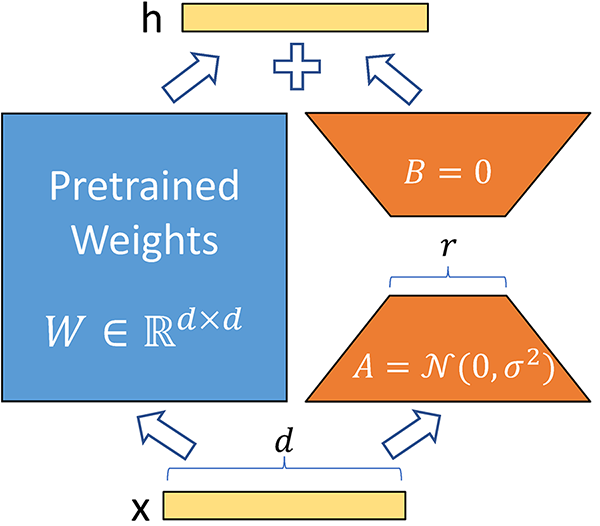
\includegraphics[width=0.5\textwidth]{images/gambar_II_8_lora.png}
  \caption{Reparameterisasi LoRA: bobot \textit{pretrained} dibekukan dan hanya matriks A dan B yang dilatih \parencite[sumber:][]{hu2021}}
  \label{fig:lora}
\end{figure}

% ============================================================================================
% II.10 Metrik evaluasi
% ============================================================================================
\section{Metrik Evaluasi dan Uji Statistik}
Akurasi pengenalan kata adalah persentase percobaan yang tebakannya benar.
Karena jumlah percobaan tiap kata bisa berbeda, \textit{balanced accuracy} memakai rata-rata ketepatan untuk setiap kata, seperti pada Persamaan~\ref{eq:bacc} \parencite{zhou2025}.
Pada persamaan tersebut, $C$ adalah jumlah kata, $TP_i$ adalah jumlah percobaan kata ke-$i$ yang ditebak benar, dan $FN_i$ adalah jumlah percobaan kata ke-$i$ yang ditebak sebagai kata lain.
\begin{equation}
\text{B-Acc} = \frac{1}{C} \sum_{i=1}^{C} \frac{TP_i}{TP_i + FN_i}
\label{eq:bacc}
\end{equation}
\eqcaption{\textit{Balanced accuracy}}

Pada model vektor makna, kata yang ditebak dipilih dari kata dengan \textit{cosine similarity} (Persamaan~\ref{eq:cosine}) tertinggi terhadap vektor prediksi.
Dengan cara ini, model vektor makna dan model klasifikasi dapat dibandingkan memakai akurasi yang sama.
Nilai \textit{cosine similarity} juga dapat dilaporkan sebagai tingkat kedekatan antara tebakan dan kata yang dimaksud.

Pengujian dilakukan dalam dua skema.
Pada skema per subjek, model dilatih dan diuji pada data subjek yang sama.
Pada skema lintas subjek, model dilatih pada data semua subjek kecuali satu, lalu diuji pada subjek yang tidak dipakai tersebut, dan langkah ini diulang bergantian untuk setiap subjek.

Perbandingan antar model diuji dengan uji Wilcoxon \textit{signed-rank}.
Uji ini membandingkan dua model pada subjek-subjek yang sama dengan melihat selisih hasilnya dan peringkat selisih tersebut, tanpa mengandaikan bahwa selisihnya tersebar normal \parencite{wilcoxon1945}.
Untuk proporsi teks yang dinilai sesuai oleh penilai manusia, dipakai uji proporsi yang membandingkan persentase yang diamati dengan persentase yang diharapkan bila hanya menebak.
Perbedaan dianggap signifikan bila nilai $p$ kurang dari 0,05.

% ============================================================================================
% II.11 Penelitian terkait
% ============================================================================================
\section{Penelitian Terkait}
Penelitian \textit{imagined speech} berbasis EEG sebagian besar memakai klasifikasi ke daftar kata tetap \parencite{lopezbernal2022}.
Pada \textit{dataset} BCIC2020-3 dengan lima kata, model klasifikasi terbaru yang dilaporkan \textcite{zhou2025} mencapai \textit{balanced accuracy} sekitar 60 persen.
Hasil untuk pengenalan banyak kata atau fonem secara umum sangat beragam dan peka terhadap rancangan \textit{dataset} \parencite{duhair2026}.

Di sisi lain, pemetaan sinyal otak ke vektor makna sudah diteliti.
\textcite{pereira2018} dan \textcite{tang2023} melakukannya pada data fMRI.
Untuk EEG \textit{imagined speech}, NeuroSpeak \parencite{neurospeak2026}, yang dipresentasikan pada ICLR 2026, menghasilkan kalimat \textit{imagined speech} dari EEG pada korpus CHISCO dengan lebih dari 20.000 kalimat, dan mencapai skor kemiripan semantik 47,70 persen pada evaluasi lintas subjek.
Ringkasan penelitian terkait ditunjukkan pada Tabel~\ref{tab:penelitian-terkait}.

\begin{table}[t]
  \centering
  \caption{Ringkasan penelitian terkait}
  \label{tab:penelitian-terkait}
  \small
  \begin{tabularx}{\textwidth}{| Y | Y | Y | Y | Y |}
    \hline
    \textbf{Penelitian} & \textbf{Sinyal dan tugas} & \textbf{Pendekatan} & \textbf{Catatan hasil} & \textbf{Perbedaan dengan penelitian ini} \\
    \hline
    NeuroSpeak (ICLR 2026) & EEG, \textit{imagined speech} tingkat kalimat (CHISCO) & Penyelarasan EEG ke \textit{embedding} bahasa, lalu dekoder teks & Kemiripan semantik 47,70\% pada evaluasi lintas subjek & Penelitian ini memakai kosakata kecil dan membandingkannya langsung dengan klasifikasi \\
    \hline
    \textcite{zhou2025} & EEG, klasifikasi \textit{imagined speech} lima kata (BCIC2020-3) & Model fondasi EEG dengan klasifikasi & \textit{Balanced accuracy} 0,6004 & Keluarannya label diskrit, sedangkan penelitian ini memetakan ke vektor makna \\
    \hline
    \textcite{tang2023} & fMRI, rekonstruksi bahasa berkelanjutan & \textit{Decoder} berbasis makna dengan model bahasa & Rangkaian kata sesuai dengan makna ucapan yang dibayangkan & Memakai fMRI, bukan EEG \\
    \hline
    \textcite{mokady2021} & Gambar, pembuatan keterangan gambar & Jaringan pemeta dari \textit{embedding} CLIP ke \textit{prefix} GPT-2 & Berhasil walaupun hanya jaringan pemeta yang dilatih & Bukan sinyal otak, menjadi dasar penggunaan \textit{adapter} \\
    \hline
    \textcite{zanini2018} & EEG, \textit{motor imagery} dan ERP & Pemusatan data berbasis geometri Riemann & Data antar subjek menjadi lebih mudah dibandingkan & Belum diterapkan pada \textit{imagined speech} \\
    \hline
    \textcite{pereira2018} & fMRI, makna kalimat & Pemetaan ke ruang semantik & Mengenali makna kalimat baru yang tidak muncul saat pelatihan & Memakai fMRI, bukan EEG \\
    \hline
  \end{tabularx}
\end{table}

Berdasarkan penelitian terkait tersebut, terdapat tiga celah yang diangkat dalam proposal ini.
Pertama, penyeragaman sinyal dengan RCT untuk pemetaan EEG \textit{imagined speech} ke vektor makna lintas subjek belum ditemukan pada literatur yang ditelaah dalam studi ini.
Kedua, perbandingan langsung antara pemetaan ke vektor makna dan klasifikasi ke label kata pada data dan pembagian data yang sama belum ditemukan pada literatur yang ditelaah.
Ketiga, penggunaan vektor makna hasil pemetaan EEG sebagai \textit{soft prompt} untuk LLM melalui \textit{adapter}, dengan LoRA sebagai cadangan, belum ditemukan pada literatur yang ditelaah.
